\documentclass[paper=letter,11pt]{scrartcl}

\KOMAoptions{headinclude=true, footinclude=false}
\KOMAoptions{DIV=14, BCOR=5mm}
\KOMAoptions{numbers=noendperiod}
\KOMAoptions{parskip=half}
\addtokomafont{disposition}{\rmfamily}
\addtokomafont{part}{\LARGE}
\addtokomafont{descriptionlabel}{\rmfamily}
%\setkomafont{pageheadfoot}{\normalsize\sffamily}
\setkomafont{pagehead}{\normalsize\rmfamily}
%\setkomafont{publishers}{\normalsize\rmfamily}
\setkomafont{caption}{\normalfont\small}
\setcapindent{0pt}
\deffootnote[1em]{1em}{1em}{\textsuperscript{\thefootnotemark}\ }


\usepackage{amsmath}
\usepackage[varg]{txfonts}
\usepackage[T1]{fontenc}
\usepackage{graphicx}
\usepackage{xcolor}
\usepackage[american]{babel}
% hyperref is needed in many places, so include it here
\usepackage{hyperref}

\usepackage{xspace}
\usepackage{multirow}
\usepackage{float}


\usepackage{braket}
\usepackage{bbm}
\usepackage{relsize}
\usepackage{tcolorbox}

\def\ketY{\ensuremath{\ket {\Psi}}}
\def\iGeV{\ensuremath{\textrm{GeV}^{-1}}}
%\def\mp{\ensuremath{m_{\textrm{proton}}}}
\def\rp{\ensuremath{r_{\textrm{proton}}}}
\def\me{\ensuremath{m_{\textrm{electron}}}}
\def\aG{\ensuremath{\alpha_G}}
\def\rAtom{\ensuremath{r_{\textrm{atom}}}}
\def\rNucl{\ensuremath{r_{\textrm{nucleus}}}}
\def\GN{\ensuremath{\textrm{G}_\textrm{N}}}
\def\ketX{\ensuremath{\ket{\vec{x}}}}
\def\ve{\ensuremath{\vec{\epsilon}}}


\def\ABCDMatrix{\ensuremath{\begin{pmatrix} A &  B  \\ C  & D \end{pmatrix}}}
\def\xyprime{\ensuremath{\begin{pmatrix} x' \\ y' \end{pmatrix}}}
\def\xyprimeT{\ensuremath{\begin{pmatrix} x' &  y' \end{pmatrix}}}
\def\xy{\ensuremath{\begin{pmatrix} x \\ y \end{pmatrix}}}
\def\xyT{\ensuremath{\begin{pmatrix} x & y \end{pmatrix}}}

\def\IMatrix{\ensuremath{\begin{pmatrix} 0 &  1  \\ -1  & 0 \end{pmatrix}}}
\def\IBoostMatrix{\ensuremath{\begin{pmatrix} 0 &  1  \\ 1  & 0 \end{pmatrix}}}
\def\JThree{\ensuremath{\begin{pmatrix}    0 & -i & 0  \\ i & 0  & 0 \\ 0 & 0 & 0 \end{pmatrix}}} 
\def\JTwo{\ensuremath{\begin{bmatrix}    0 & 0 & -i  \\ 0 & 0  & 0 \\ i & 0 & 0 \end{bmatrix}}}
\def\JOne{\ensuremath{\begin{bmatrix}    0 & 0 & 0  \\ 0 & 0  & -i \\ 0 & i & 0 \end{bmatrix}}}
\def\etamn{\ensuremath{\eta_{\mu\nu}}}
\def\Lmn{\ensuremath{\Lambda^\mu_\nu}}
\def\dmn{\ensuremath{\delta^\mu_\nu}}
\def\wmn{\ensuremath{\omega^\mu_\nu}}
\def\be{\begin{equation*}}
\def\ee{\end{equation*}}
\def\bea{\begin{eqnarray*}}
\def\eea{\end{eqnarray*}}
\def\bi{\begin{itemize}}
\def\ei{\end{itemize}}
\def\fmn{\ensuremath{F_{\mu\nu}}}
\def\fMN{\ensuremath{F^{\mu\nu}}}
\def\bc{\begin{center}}
\def\ec{\end{center}}
\def\nus{$\nu$s}

\def\adagger{\ensuremath{a_{p\sigma}^\dagger}}
\def\lineacross{\noindent\rule{\textwidth}{1pt}}

\newcommand{\multiline}[1] {
\begin{tabular} {|l}
#1
\end{tabular}
}

\newcommand{\multilineNoLine}[1] {
\begin{tabular} {l}
#1
\end{tabular}
}



\newcommand{\lineTwo}[2] {
\begin{tabular} {|l}
#1 \\
#2
\end{tabular}
}

\newcommand{\rmt}[1] {
\textrm{#1}
}


%
% Units
%
\def\m{\ensuremath{\rmt{m}}}
\def\GeV{\ensuremath{\rmt{GeV}}}
\def\pt{\ensuremath{p_\rmt{T}}}


\def\parity{\ensuremath{\mathcal{P}}}

\usepackage{cancel}
\usepackage{ mathrsfs }
\def\bigL{\ensuremath{\mathscr{L}}}

\usepackage{ dsfont }



\usepackage{fancyhdr}
\fancyhf{}


\lhead{\Large 33-444} % \hfill Introduction to Particle Physics \hfill Spring 2022}
\chead{\Large Introduction to Particle Physics} % \hfill Spring 2022}
\rhead{\Large Spring 2022} % \hfill Introduction to Particle Physics \hfill Spring 2022}
\begin{document}
\thispagestyle{fancy}





%\begin{tabular}{c}
%{\large 33-444 \hfill Intro To Particle \hfill Spring 2022\\}
%\hline 
%\end{tabular}

\begin{center}
{\huge \textbf{Homework Set \#8 }}
\large

{\textbf{ Due Date:} *Monday* April 11th  } 
\end{center}

{\large


\textbf{1)  $W$ boson decays to electrons. } \hfill \textit{(3 points)}\\
\begin{itemize}
\item[a)]{ The W can decay directly to an electron or to electron by decaying through a $\tau$. Draw the corresponding diagrams.}
\item[b)]{ Estimate how often the W decays to an electron. }
\end{itemize}           

\vspace*{0.25in}

\textbf{2) Higgs Boson Decays. } \hfill \textit{(3 points)}\\
The Higgs boson decays at a high rate to pairs of W-bosons.
A clean way to observe this signal is in the $e\mu$ + Missing transverse energy final state. How often do $H\rightarrow WW$ events lead to a $e\mu$ final state?

\vspace*{0.25in}


\textbf{2) Tracking Detectors } \hfill \textit{(10 points)}\\

Consider a charged particle emitted from a high-energy interaction, moving through a cylindrical tracking chamber of radius L under the influence of a solenoidal magnetic field B. 
Assume that the particle moves in a plane perpendicular to the axis of the cylinder and the direction of the magnetic field.
\begin{itemize}
\item[a)]{
Because the initial direction of the particle is not a priori known, the curvature is measured from the sagitta s of its curved trajectory, defined to be the maximum deviation of the curve from a straight line between the point of origin and the point where the particle exits the detector at radius L.
Show that, for small curvature, s = $\frac{qBL^2}{8p_T}$.}
\item[b)]{
If $\Delta s$ is the uncertainty in the measurement of the sagitta, derive the formula for $\frac{\Delta p_T}{p_T}$ in terms of $p_T$, L, B, and $\Delta s$.
}
\item[c)]{
It can be shown that, if the tracking detector makes N equally spaced position measurement, each with resolution $\epsilon$, the uncertainty in the measurement of the sagitta is
\be
\Delta s = \frac{3.4 \epsilon }{\sqrt{N + 5}}
\ee
For N = 50, $\epsilon$ = 100 $\mu m$, L = 1 m, and B = 1 T, estimate the uncertainty in the obtained value of $p_T$.
}
\end{itemize}

\vspace*{0.25in}

\textbf{3) Limits of the Tracking System.} \hfill \textit{(5 points)}\\

The tracking system at ATLAS is a cylinder with an outer radius of 1.1 meters which contains a 2 T solenoidal magnetic field, ie., the magnetic field lines are parallel to the axis of the cylinder. 
Immediately outside of the tracking system is a region of 0 magnetic field, where the electromagnetic calorimeter is located.

\begin{itemize}
\item[a)]{
The energy of charged particles that do not leave the tracking system is poorly measured because those particles do not reach the calorimetry. 
Estimate the minimum $p_T$ in GeV for an electron to reach the calorimetry.
}

\item[b)]{
The semiconductor tracker is a subsystem of the tracker that is also a cylinder, but with an outer radius of 0.5 meters. 
It consists of layers of silicon that can measure particle positions accurate to 17 micrometers. 
Extremely high energy charge particles do not bend enough in the magnetic field to have their charge accurately measured. 
Estimate the maximum $p_T$ in GeV of a muon that the semiconductor tracker can determine bent in the magnetic field.
}
\item[c)]{
For a high $p_T$ track that just bends in this magnetic field, what is the uncertainty in the measurement of the $p_T$? Estimate this using the resolution of the silicon tracking system.
}
\end{itemize}

\vspace*{0.25in}

\textbf{4) Rapidity.} \hfill \textit{(15 points)}\\

\begin{itemize}
\item[a)]{
In experimental particle physics, it is often very useful to express the direction of motion of a particle in terms of its rapidity y. The rapidity is defined as
\be
y = \frac{1}{2} log \frac{E+p_z}{E - p_z}
\ee
for a particle with energy E and z-component of momentum $p_z$. 
What makes rapidity so nice is its simple properties under Lorentz transformation. 
Perform a Lorentz boost of the energy and momentum along the z-axis with velocity $\beta$. 
How does the rapidity transform under this boost? 
}
\item[b.]{
The pseudorapidity $\eta$ is defined as $\eta = - \ln \tan \frac{\theta}{2}$ where the polar angle is $\theta$ from the beam axis.
Pseudorapidity is 0 for particles moving directly perpendicular to the beam at the interaction point. It is $\pm \infty$ along the proton beams where the polar angle is $0$ or $\pi$. 
For a mass-less particle,  the polar angle is$\ \cos \theta = p_z/E$.
How does rapidity y depend on pseudorapidity $\eta$ for mass-less particles?
Any massless four-vector p can be expressed in $(\eta, \phi, p_T)$ coordinates as $p = p_T(\cosh \eta, \cos \phi,  \sin \phi, \sinh \eta)$
}
\item[c.]{

The Figure is an event display from the ATLAS experiment. 
The large image is a head-on view of the ATLAS experiment, with the tracker, calorimeters, and muon system visible. 
At the lower right, is a so-called “Lego plot.” 
This “unrolls” the detector, and displays the distribution of $p_T$ deposited in the $(\eta, \phi)$ plane.

\begin{figure}[h!]
\centering
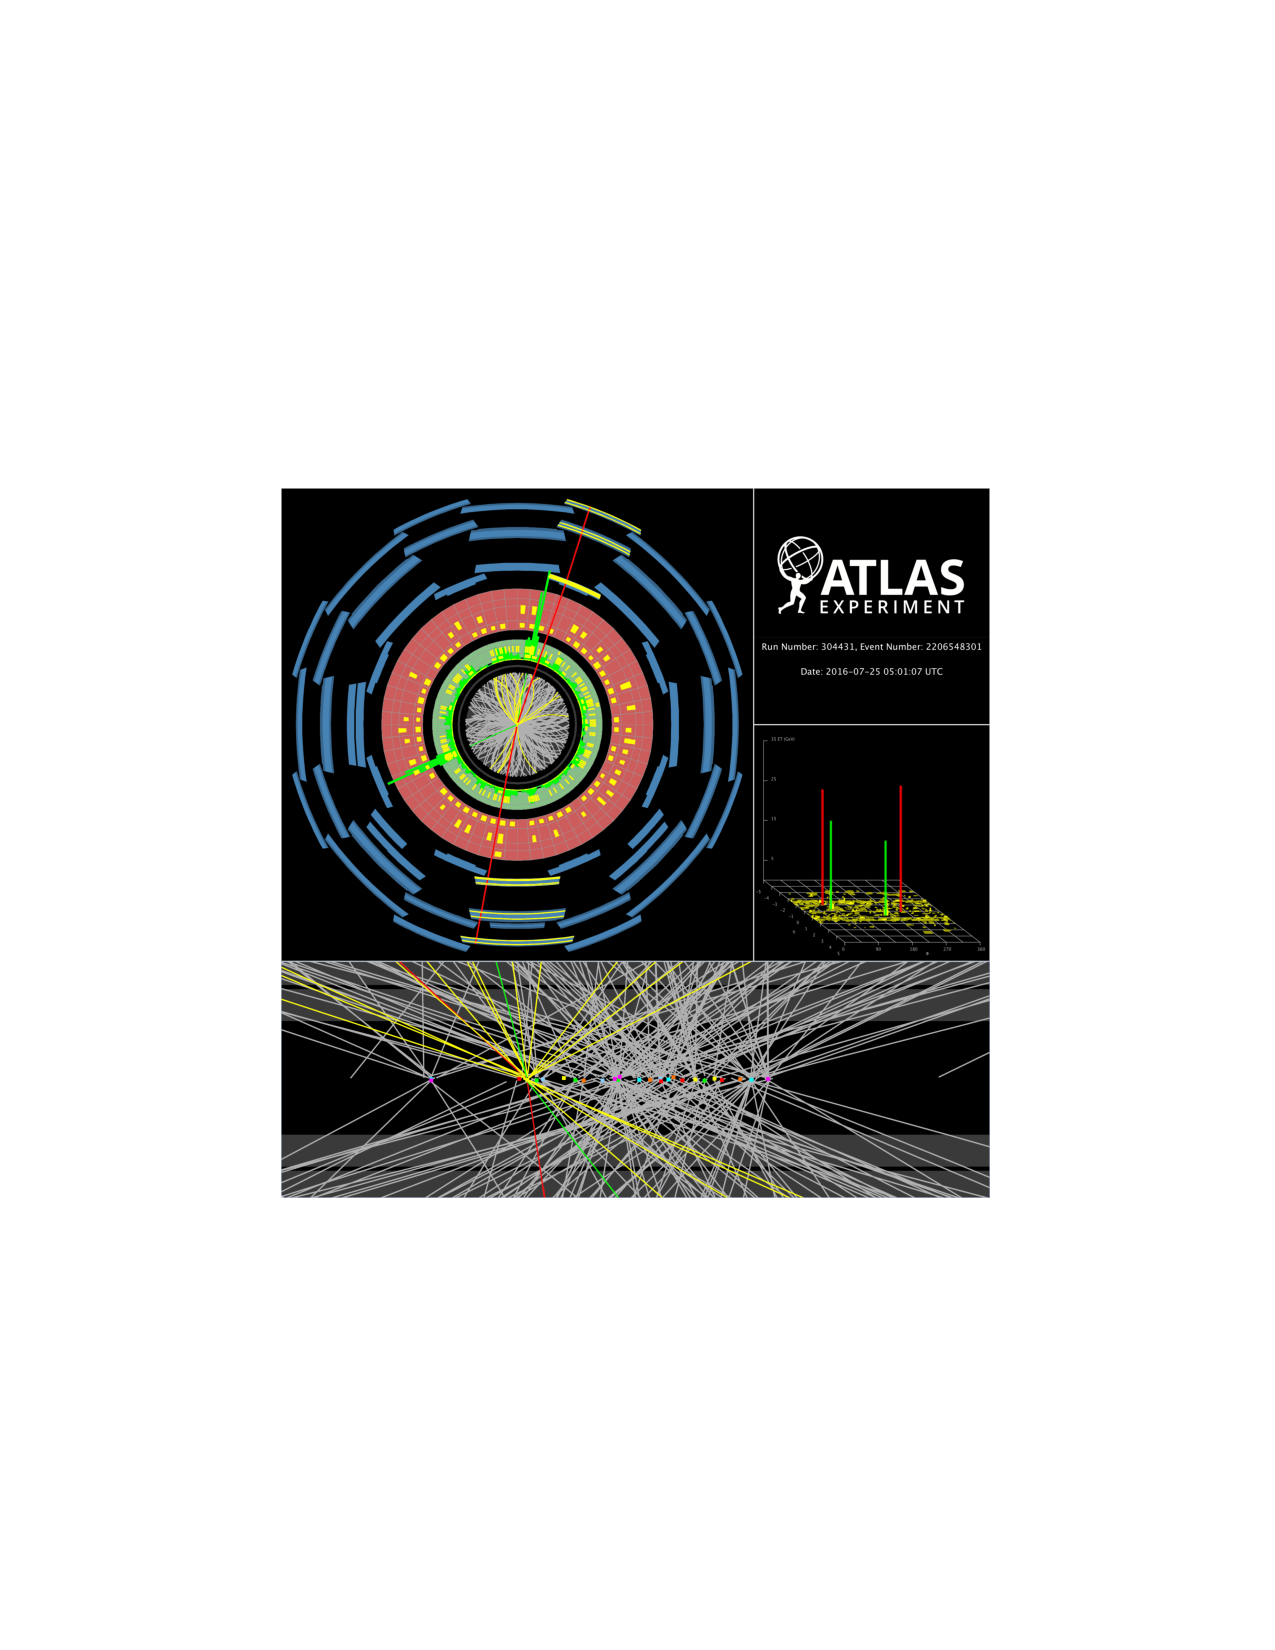
\includegraphics[width=0.8\textwidth]{./EventDisplay.pdf}
\end{figure}

\item[d.]{ Based on the “hits” in the tracker, EM calorimeter, hadronic calorimeter, and muon system, identify the particle type of the red and green spike in the Lego plot. 
Both red particles are identical as are both green particles.}
\item[e.]{
From the Lego plot, determine the four-vectors of each of the red and green particles. 
A zoomed in view of the Lego plot is also provided. You can safely neglect the particles’ masses. 
}
\item[f.]{
What is the total transverse momentum vector of the four particles?
}
\item[h.]{What is the invariant mass of red particles together? }
\item[i.]{What is the invariant mass of green particles together? }
\item[j.]{What is the invariant mass of all particles together ? Which particle of the Standard Model does this mass correspond most closely to?}

\begin{figure}[h!]
\centering
\includegraphics[width=0.8\textwidth]{./EventDisplayZoom.pdf}
\end{figure}

}

\end{itemize}




\end{document}
